\documentclass[11pt]{article}

% Target venue: Mountain Research and Development (MRD), MountainResearch
% section. Constraints: 4,000 words max excluding references; abstract
% 150-300 words single paragraph; up to 3 heading levels; must state
% transferability to other mountain regions. See PLAN.md.

\usepackage[margin=1in]{geometry}
\usepackage{amsmath,amssymb}
\usepackage{graphicx}
\usepackage{xcolor}
\usepackage{booktabs}
\usepackage[colorlinks=true,linkcolor=blue,citecolor=blue,urlcolor=blue]{hyperref}
\usepackage{natbib}
\setcitestyle{authoryear,open={(},close={)}}

\title{FLOW: An Open-Data Workflow for Flash Flood Early Warning in Nepal's Koshi Basin}

\author{
  Saurab Dulal \and Sanjeeb Prasad Panday
}

\date{}

\begin{document}

\maketitle

\begin{abstract}
Flash floods are among Nepal's most destructive hazards, where more than 6,000 rivers drain steep, monsoon-fed catchments into densely populated floodplains. Effective early warning requires integrating hazard monitoring, statistical flood prediction, and spatial visualization, yet most operational systems (the US NWS FFMP, the Central America Flash Flood Guidance System) are built for large, well-instrumented regions and do not transfer to small, data-scarce mountain basins. This paper presents FLOW, a low-cost, open-data workflow for Nepal's Koshi Basin that combines satellite rainfall estimation, flood frequency analysis (Gumbel's and Log-Pearson Type III methods), and GIS-based flood inundation mapping. We describe FLOW's architecture and methodology, and report flood-frequency and inundation-extent results built entirely on hydro-meteorological records for the basin's Sunkoshi and Saptakoshi gauges together with free, open global datasets: a Copernicus GLO-30 DEM, GPM IMERG satellite rainfall, GloFAS discharge reanalysis, and a Height Above Nearest Drainage (HAND) inundation model. A comparison of monthly rainfall against monthly discharge over their 297 months of overlap shows the two independently-sourced open datasets track each other closely (Pearson r=0.84 at zero lag, rising to r=0.85 at a one-month lag, both p$<$10$^{-75}$), a real cross-check of the pipeline's internal consistency rather than a validation against ground truth. Separately, checking our GloFAS-derived discharge series directly against an independently published gauge-based figure for the Koshi at Chatara finds it running about 76\% high in the one year we could directly compare, even though its long-run mean is within about 22\% of the published mean annual flood discharge --- a specific, demonstrated limitation of GloFAS-based single-point extraction for this basin that we report as a caution for similar small-basin studies, rather than as a validated basis for the design-flood values in this paper. We situate this against a decade of literature on satellite rainfall products, machine-learning-based forecasting, and Nepal-specific GIS flood-mapping studies, and motivate continued relevance with two 2026 events: a catastrophic glacial-collapse flood on the Trishuli River, and a live alert-level bulletin for the Sun Koshi itself. Because the workflow relies only on globally-available open data and software, it is directly transferable to other data-scarce mountain basins beyond Nepal.

\medskip
\noindent\textbf{Keywords:} flash flood, early warning system, flood frequency analysis, GIS, HAND, satellite rainfall, Nepal, Koshi Basin
\end{abstract}

\section{Introduction}

Nepal ranks 12th globally by population share exposed to annual flood risk (23.74\%) \citep{undp2004}, and floods/landslides account for an estimated 29\% of annual disaster deaths and 43\% of disaster-related property loss \citep{dwidp2004}. The Terai, home to roughly half the national population on 17\% of its land, bears the brunt. Two events illustrate the danger: the May 2012 Seti River flash flood in Kaski district (a landslide-dammed lake outburst, $\geq$31 deaths), and the \textbf{August 18, 2008} Koshi River embankment breach at Kusaha, Sunsari district --- UN OCHA situation reports \citep{ocha2008koshi} confirm this date and displacement figures of 66,500--70,000 people domestically (over 400 died in Bihar, India), matching village-level detail (Sripur, Haripur, Paschim/West Kusaha) from the affected area.

Flash floods differ from ordinary floods in speed: a rapid rise within hours of a trigger (intense rainfall, glacial lake outburst, landslide-dam failure), leaving little time for manual response. The United Nations' four-element early-warning model --- risk knowledge, monitoring/forecasting, dissemination, response capability \citep{un2006} --- is hard to satisfy in mountain basins because of sparse instrumentation and steep, glacier- and landslide-influenced catchments where the trigger \emph{type} is itself variable and hard to anticipate. This basic architecture recurs, in variously adapted forms, across the regional literature on flash-flood guidance system design \citep{grabs2010} and event-specific early-warning-system case studies \citep{konarik,kundzewicz}.

This still matters, nationally and in this paper's specific study basin alike. On 26 August 2026, a Langtang Lirung glacier collapse produced a catastrophic debris flow on the Trishuli River in Rasuwa district (fed by a Bhote Koshi originating near Gyirong/Kerung, Tibet, part of the Gandaki/Narayani drainage, hydrologically separate from this paper's Sun Koshi/Saptakoshi study basin), with reported deaths ranging ${\sim}$1,200--1,369 and missing ${\sim}$4,200--5,100 as of early September 2026 \citep{usgs2026,unfpa2026} (figures still being reconciled at time of writing). Reporting indicates a rapid, multi-meter rise in river level within tens of minutes, a failure mode that rainfall-threshold-based monitoring is poorly suited to catch, since it originates from glacial/mass-wasting processes rather than precipitation. The WMO \citep{wmo2026} has since observed this was the \emph{second} major flood in fourteen months on the same Lhende Khola tributary, underscoring a recurring, not one-off, monitoring gap, and Nature India \citep{natureindia2026} has directly editorialized that earlier warning could have saved hundreds of lives. \emph{(Some domestic reporting also attributes flood casualties in Sindhupalchok district, on the Sun Koshi system's own Bhote Koshi tributary near Barhabise, to this same date; whether that reflects a second, distinct event on this paper's actual study basin or a misattribution across Nepal's two identically-named ``Bhote Koshi'' rivers could not be confirmed from available primary sources at time of writing, so it is noted here but not relied upon anywhere in this paper.)}

The Sun Koshi basin itself remains under live, present-day flood risk independent of that question: on \textbf{2 September 2026} (around 06:50--07:02 local time), DHM's Flood Forecasting Division issued a special bulletin reporting the Sun Koshi's water level at Khurkot, Sindhuli, upstream of both gauge stations examined in this paper, crossing its official alert threshold (7.69\,m against a 7.5\,m alert level / 8.6\,m danger level) amid continuous monsoon rainfall \citep{dhm2026bulletin}, prompting a caution notice for downstream riverine communities in Sindhuli and Ramechhap districts. Monitoring and frequency-based prediction that generalizes across trigger types, glacial/mass-wasting events as well as ordinary monsoon-driven flooding, remains a live need for exactly this basin, not just a general national statistic.

\subsection{Existing systems and the gap FLOW occupies}

The US relies on weather radar feeding NWS's Flash Flood Monitoring and Prediction system; the Central America Flash Flood Guidance System (CAFFG, post-Hurricane Mitch) centralizes real-time rainfall ingestion, soil-moisture/threshold-runoff modeling, and dissemination across seven countries \citep{gourley2022}. At the community scale, Mercy Corps' work in Kailali district, Nepal established a manually-read gauge network and a community communication tree \citep{smith2017communitybased}, but with no integrated statistical prediction or spatial flood-mapping capability. Between expensive centralized infrastructure and manual observation lies a gap: a low-cost, desktop-deployable tool that a single technical team (a DHM office, an NGO, a university department) could run for one basin at a time, combining statistical flood prediction with GIS-based spatial visualization. FLOW occupies that gap. \emph{(We call this paper's contribution FLOW because this paper implements and evaluates the open-data prediction module, flood frequency analysis and GIS-based mapping, not the full early-warning system with its SMS dissemination and visualization interface, which remains part of FFEWS's original design and is not re-implemented here; see Section~3.)}

\textbf{Contribution.} (1) We present the architecture and methodology of FLOW, an open-data implementation of the prediction module from the original FFEWS concept, integrating satellite rainfall estimation, flood frequency analysis, and GIS-based flood mapping for the Koshi Basin. (2) We describe a fully open-data, open-source implementation of this methodology, real terrain, real satellite rainfall, and a HAND-based inundation model, that requires no licensed GIS software. (3) We report flood-frequency and inundation-extent results for the basin's Sunkoshi/Saptakoshi gauges, including goodness-of-fit statistics and a three-method comparison (Gumbel, Log-Pearson III, GEV), illustrative of the workflow's output rather than validated design-flood values, for reasons given in Section~5.1. (4) We cross-validate the rainfall and discharge datasets against each other over their period of overlap as an internal-consistency check. (5) We situate this work against the substantial post-2016 literature on satellite rainfall, ML-based flash-flood forecasting, and Nepal-specific GIS flood-mapping studies. (6) We check our GloFAS-derived discharge series against an independently published discharge figure for the Koshi at Chatara and find a substantial high bias in the one directly comparable year available, a specific, actionable caution for other GloFAS-based single-point-extraction studies on small basins, not merely a generic reanalysis disclaimer. (7) We state explicit transferability of this workflow to other mountain regions.

\section{Related Work}

\noindent\textbf{Operational flash-flood guidance systems.} The FFMP/ALERT model (USA) and CAFFG (Central America) remain the reference architectures for centralized flash-flood guidance: real-time rainfall ingestion, soil-moisture and threshold-runoff modeling, and automated dissemination. \citet{gourley2022} document the multi-decadal expansion of this system family into a globally-deployed Flash Flood Guidance System (FFGS) under WMO coordination --- Nepal is not yet a full FFGS participant region, which is part of the motivation for basin-scale tools like FLOW.

\noindent\textbf{Community-based early warning.} Mercy Corps' Kailali district program \citep{smith2017communitybased} demonstrates that even manual gauge-reading and a well-designed communication tree can meaningfully reduce response time, but such systems provide no statistical basis for anticipating flood magnitude or extent --- a gap FLOW's frequency-analysis and mapping modules are designed to fill.

\noindent\textbf{Satellite rainfall estimation, post-TRMM.} GPM IMERG has become the standard successor to TRMM-era rainfall products, with several validation studies specifically over Nepal and the Himalaya \citep{atmosphere2021,remotesensing2022,remotesensing2020,jhydrology2021,ees2025}.

\noindent\textbf{Machine-learning-based flash flood forecasting.} A substantial post-2020 literature has moved beyond pure statistical/empirical methods \citep{water2024review,intelligentflood2023,lesvos2023}, comparable in scope to FLOW but using modern deep learning rather than Gumbel/Log-Pearson frequency analysis.

\noindent\textbf{GIS/HEC-RAS flood mapping in Nepal.} Most directly relevant to this paper, \citet{sharma2025westrapti} appraise flood risk and inundation extent in the West Rapti River Basin, Nepal, using Gumbel's method for frequency analysis feeding 2D HEC-RAS hydraulic modeling and GIS-based mapping on real Nepal terrain and discharge data throughout. A 2026 Roshi Basin study \citep{roshi2026} and other South Asian HEC-RAS 2D applications \citep{pandit2023kamla,vashist2023krishna} further establish this as a well-trodden and validated regional methodology.

\section{System and Methods}

The original FFEWS concept (2014) was designed around three modules: a \textbf{prediction module} (satellite rainfall estimation + flood frequency analysis), a \textbf{warning/communication module} (SMS-based dissemination), and a \textbf{visualization module} (interactive time-series and map-based views), backed by a historical hydro-meteorological database and a real-time monitoring feed from DHM's public data pages. This paper re-implements and reports results for the prediction module only, as an open-data pipeline we call \textbf{FLOW}: the analysis and results reported in Sections~4--5 concern flood frequency and inundation mapping specifically; the warning/communication and visualization modules are part of FFEWS's original design and are not re-tested or re-implemented here.

\subsection{Satellite Rainfall Estimation}
Cloud-top brightness temperature $T$ (K) is related to rainfall rate $R$ (mm/h) via the standard geostationary-IR empirical form
\begin{equation}
R = 1.1183\times10^{11}\exp\left(-3.6382\times10^{-2}T^{0.5}\right),
\end{equation}
with adjustments for precipitable water and surface relative humidity. Satellite imagery is pixel-processed to estimate rainfall over the area of interest and compared against critical rainfall thresholds to trigger warnings. In the workflow reported here, this module's role is served operationally by GPM IMERG (Section~4).

\subsection{Flood Frequency Analysis}
FFA predicts design-flood discharge at a range of return periods from a series of annual maximum flows. FLOW implements two standard methods, among several surveyed but not implemented for ungauged basins (Snyder's, B.D.\ Richard's, Modified Dicken's):
\begin{itemize}
\item \textbf{Gumbel's method}: treats the annual maximum daily flow as an extreme-value variate; return-period discharge is computed as $x_T=\bar{x}+K\sigma_X$ with the frequency factor $K$ derived from the reduced variate $Y_T=-\ln(\ln(T/(T-1)))$.
\item \textbf{Log-Pearson Type III}: log-transforms the discharge series ($z=\log x$), computes the skew coefficient $C_s$ of the log-series, and derives return-period discharge as $z_T=\bar{z}+K_z\sigma_z$, with $x_T=\mathrm{antilog}(z_T)$.
\end{itemize}
Both methods are applied at return periods of 1.01, 2, 5, 10, 25, 50, 100, and 200 years.

\subsection{Flood Map Generation}
Inundation mapping proceeds in four conceptual stages: (I) deriving a river centerline, bank lines, and cross-sections from a DEM, with channel roughness assigned per reach; (II) a steady-flow hydraulic solve for a given discharge boundary condition; (III) converting the resulting water surface into an inundation extent over the DEM; and (IV) overlaying aerial/satellite imagery for interpretation of affected areas. Section~4.2 describes the specific open-source implementation of this pipeline used in this study.

\section{Data}

\subsection{Hydro-meteorological records}
Discharge and rainfall data come from the Koshi Basin's DHM gauge network. \textbf{Station 681} is the Sunkoshi River gauge at Hampachuwar (26$^\circ$55$'$39.86$''$N, 87$^\circ$08$'$35.05$''$E, elevation 116\,m, 18,164\,km$^2$ drainage, published record 1991--2019); \textbf{station 695} is the Saptakoshi River gauge at Chatara (26$^\circ$51$'$19.98$''$N, 87$^\circ$08$'$58.72$''$E, 53,686\,km$^2$ drainage, published record 1977--2023) --- the basin's outlet gauge \citep{dhm2025stationlist}. Neither station's digital daily record is openly downloadable: both require a formal data request through DHM's ``Request Data'' portal (dhm.gov.np/hydrology/hms-Single/207), which is precisely the kind of access barrier this workflow is designed to operate around.

\subsection{Open global datasets}
The results reported here (Section~5) therefore use free, globally-available open data throughout:

\begin{itemize}
\item \textbf{Terrain:} Copernicus GLO-30 DEM (30\,m), via the OpenTopography Global DEM API for a bounding box covering the study reach around Hampachuwar and Chatara (26.70--27.00$^\circ$N, 87.00--87.40$^\circ$E) plus a buffer.
\item \textbf{Rainfall:} GPM IMERG (\texttt{GPM\_3IMERGM}, monthly), 2001--2025, via NASA's \texttt{earthaccess} --- adequate for climatological comparison, though monthly resolution is not sufficient for sub-daily rainfall-runoff forecasting (Section~6).
\item \textbf{Discharge:} GloFAS (Global Flood Awareness System) historical reanalysis, 1979--2025, via the CEMS Early Warning Data Store's API. This is \textbf{model reanalysis output (LISFLOOD forced by ERA5), not an observed gauge record}, a limitation stated plainly here; an observed gauge record would supersede it as the primary discharge source. Single-point extraction requires a window search rather than nearest-neighbor lookup: GloFAS's ${\sim}$5\,km grid does not align exactly with the river centerline, so the cell nearest the gauge's literal coordinates falls on an adjacent hillslope pixel, returning discharge of order 1--24\,m$^3$/s, two to three orders of magnitude too small for a 53,686\,km$^2$ basin. Searching a small window around the gauge point and selecting the cell with the highest mean discharge (the main-channel signature) yields a plausible 259.5--16,951.5\,m$^3$/s range across the 47-year record. We flag this as a reusable methodological caution for other GloFAS point-extraction studies. ``Plausible'' here means order-of-magnitude sensible, not validated: Section~5.1 reports a direct check of this series against a published Chatara gauge figure that found it running substantially high in the one year directly comparable.
\item \textbf{Flood mapping:} HAND (Height Above Nearest Drainage), computed from the DEM via the open-source \texttt{pysheds} library, with a stream network delineated at a flow-accumulation threshold of 1,000 contributing cells (an unvalidated default, not tuned against any independent channel-extent reference for this basin). Return-period discharge (Section~5) is converted to an inundation depth via an empirical hydraulic-geometry power-law relation in the style of \citet{leopoldmaddock1953}, using generic literature coefficients rather than a Nepal- or Himalaya-fitted regression, and applied as a single basin-wide depth rather than one that varies with local contributing drainage area along the network. Both are real simplifications relative to a surveyed cross-section and a spatially-distributed hydraulic solve, carried through explicitly rather than hidden, and discussed further in Section~6.
\item \textbf{Gauge stage records (event corroboration only):} Nepal's BIPAD disaster portal \citep{bipad2026} (\texttt{bipadportal.gov.np}, sourced from \texttt{hydrology.gov.np}) publishes a historical archive of gauge water-level readings at ${\sim}$10-minute resolution; we retrieved the full record for both study stations, covering late 2020--2026. This is stage (m), not discharge (m$^3$/s) --- no rating curve is available to convert it --- so it is used only for the event-timing check in Section~5.1, not as a discharge source.
\end{itemize}

\section{Results}

\subsection{Flood Frequency Analysis}
Table~\ref{tab:ffa} reports return-period discharge from both methods on the full 1979--2025 discharge series (47 annual maxima). Divergence between methods is reported throughout as a percentage of the mean of the two estimates. The two methods track closely for T=2--25 years (0.2--0.7\% apart, Gumbel modestly higher through T=10 before Log-Pearson III overtakes by T=25), diverge most at the T=1.01-year extreme (5.9\% apart, Log-Pearson III higher), and diverge progressively at longer return periods, reaching a 2.8\% spread at T=200 years (Log-Pearson III higher; Figure~\ref{fig:ffa}). A Kolmogorov--Smirnov test does not reject either fit (Gumbel: D=0.092, p=0.78; Log-Pearson III: D=0.093, p=0.77), with RMSE against the empirical plotting-position discharge of 863\,m$^3$/s (Gumbel) and 774\,m$^3$/s (Log-Pearson III) --- 10.1\% and 9.1\% of the mean annual maximum (8,527\,m$^3$/s), respectively. We report this as a still-informal check rather than a fully validated fit: both methods' parameters were estimated from the same 47-point sample being tested, which is known to inflate the KS test's reported p-value relative to a fully-specified null. The Log-Pearson III skew coefficient ($C_s\approx0.42$, standard error on the order of $\sqrt{6/n}\approx0.36$ for $n=47$) is a positive estimate that, at a ratio of only ${\approx}1.2$ standard errors from zero, remains statistically indistinguishable from zero by conventional thresholds; we therefore do not treat the skew as confidently nonzero. The two methods nonetheless track closely across most of the return-period range, diverging only at the extremes.

\begin{table}[h]
\centering
\begin{tabular}{@{}lrr@{}}
\toprule
Return period (yr) & Gumbel (m$^3$/s) & Log-Pearson III (m$^3$/s) \\
\midrule
1.01 & 4,609 & 4,889 \\
2    & 8,135 & 8,093 \\
5    & 10,243 & 10,174 \\
10   & 11,639 & 11,591 \\
25   & 13,402 & 13,433 \\
50   & 14,710 & 14,847 \\
100  & 16,009 & 16,298 \\
200  & 17,303 & 17,800 \\
\bottomrule
\end{tabular}
\caption{Flood-frequency results, Sun Koshi/Saptakoshi, 1979--2025 --- illustrative of the workflow's output, not validated design-flood values (Section~5.1).}
\label{tab:ffa}
\end{table}

\begin{figure}[h]
\centering
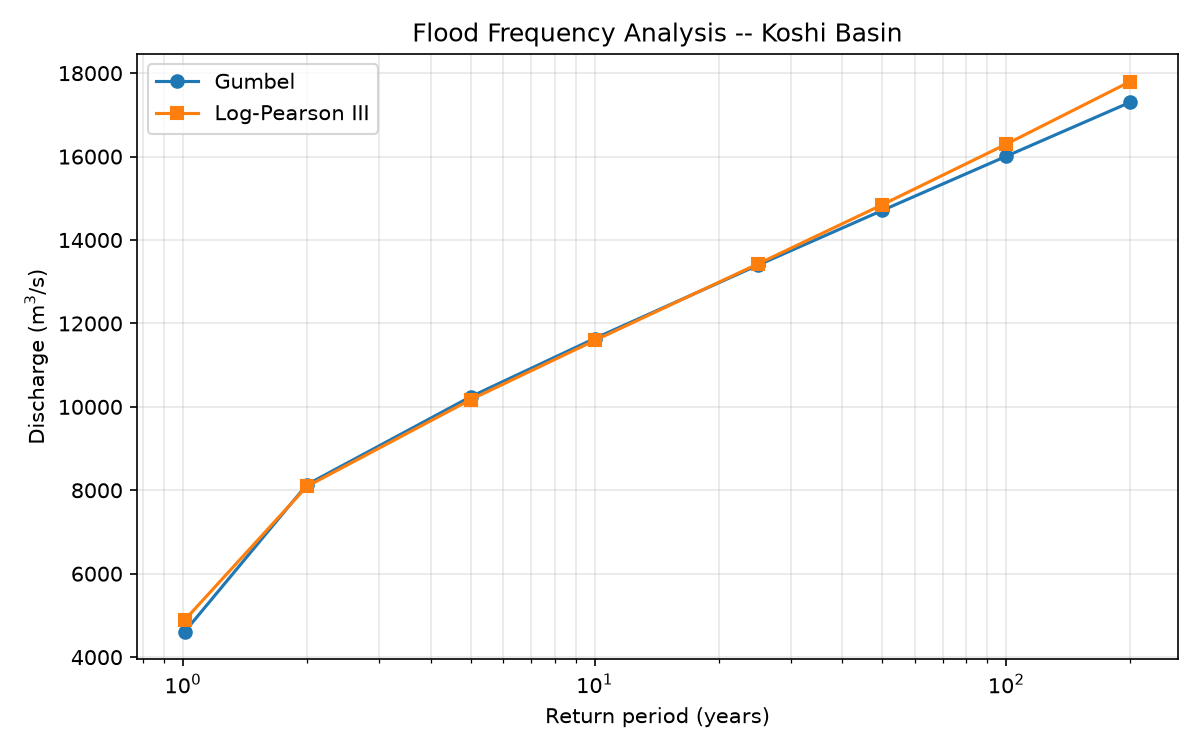
\includegraphics[width=0.85\linewidth]{../analysis/outputs/ffa_comparison_plot.png}
\caption{Flood-frequency curves (log return-period axis) for Gumbel and Log-Pearson III, corresponding to Table~\ref{tab:ffa} --- illustrative of the workflow's output, not validated design-flood values (Section~5.1).}
\label{fig:ffa}
\end{figure}

Two further caveats bear on how these numbers should be read. First, on extrapolation: the 47-year record means T=100 and T=200-year estimates extrapolate about 2.1$\times$ and 4.3$\times$ beyond the record length, respectively. Such estimates should be read with the caution standard for any flood-frequency extrapolation. The close agreement between Gumbel and Log-Pearson III across the return-period range describes the fitting procedure, not the accuracy of the discharge values themselves: it is equally consistent with both methods sharing a blind spot to the same feature of the data (see the GEV result immediately below) as with the values being correct. \emph{(A three-method comparison that also fits the Generalized Extreme Value (GEV) distribution is unusable on this series: GEV's maximum-likelihood fit is degenerate --- shape parameter ${\approx}-6.6$, with a Kolmogorov--Smirnov test rejecting the fit decisively (p${\approx}1.5\times10^{-25}$). This is driven by a cluster of the three-to-four highest years (1987: 16,951\,m$^3$/s; 2019: 15,045\,m$^3$/s; 1995: 12,881\,m$^3$/s; 2017: 12,785\,m$^3$/s) rather than any single outlier: removing 1987 alone leaves the fit almost as degenerate (shape ${\approx}-6.4$), while removing all four yields a well-behaved fit (shape ${\approx}+0.5$, KS p=0.36). Three-parameter GEV maximum-likelihood fits are known to be highly sensitive to exactly this kind of upper-tail clustering; we therefore rely on Gumbel and Log-Pearson III, which are numerically stable here --- while noting, per the point above, that their mutual agreement does not by itself establish accuracy.)} Second, and separately from record length: this analysis is built on \emph{daily} discharge, while Section~1 defines flash floods by sub-daily speed (a rise of meters within tens of minutes to hours). Table~\ref{tab:ffa}'s return-period discharges are therefore best read as conventional flood-frequency statistics, useful for hazard zoning and the inundation mapping in Section~5.3, rather than as estimates of flash-flood peak discharge specifically, which would require sub-daily observations this study does not have.

\paragraph{Checking against published discharge records.} Because no observed DHM record was available to validate the GloFAS-derived discharge series directly (Section~4.1), we instead checked it against gauge-based discharge figures for the Koshi at Chatara reported in independent published literature \citep{devkota2012koshibarrage}. This is a partial check, not a full validation, and we report it as such: only one year in our record --- 2008 --- has an unambiguous published value we could compare against directly; the paper's other reported figures (mean annual flood discharge, the 1968 historic peak) are themselves relayed by \citet{devkota2012koshibarrage} from earlier sources rather than originating there. On long-run average, our series is broadly consistent with the published record: the mean of our 47 annual maxima (8,527\,m$^3$/s) is about 22\% above the published mean annual flood discharge for the Koshi at Chatara (${\sim}$7,000\,m$^3$/s). For the one year we could check directly, however, our series runs substantially high: 2008 (our 7,482\,m$^3$/s vs.\ a published 4,250\,m$^3$/s, +76\%) (Table~\ref{tab:validation}). A single directly-comparable year cannot establish a general event-level bias, but it is enough to say plainly that we cannot currently trust this series' magnitude in any individual year, only its long-run order of magnitude. For scale, the largest flood on record at Chatara --- 1968, predating our 1979--2025 GloFAS record and not a like-for-like check --- reportedly reached 25,879\,m$^3$/s \citep{devkota2012koshibarrage}; we note this only as context for the basin's known range, not as evidence about our own series' accuracy. We read the 2008 discrepancy as a signal that GloFAS --- a global model forced by ERA5 rainfall, with no representation of the Koshi Barrage and embankments that have regulated flow at this location since 1963 --- may reproduce this basin's long-run discharge climatology better than it reproduces the magnitude of any specific event, though one comparison year cannot confirm this is systematic. Accordingly, we treat the return-period discharge values in Table~\ref{tab:ffa}, and the inundation extents derived from them in Section~5.3, as illustrating what this open-data workflow produces end-to-end, not as validated design-flood or hazard-mapping values for the Koshi Basin. We consider this check, reported with its real limits rather than overstated, a more durable contribution than the specific discharge numbers it is applied to --- and a reusable caution for other GloFAS-based small-basin studies: check every available published figure before trusting a single-point-extraction series, and expect the long-run mean to look more reasonable than any individual year does.

\begin{table}[h]
\centering
\small
\begin{tabular}{@{}lrrr@{}}
\toprule
Comparison & Published (m$^3$/s) & Our GloFAS-derived (m$^3$/s) & Difference \\
\midrule
Mean annual flood discharge (long-run) & ${\sim}$7,000 & 8,527 & +22\% \\
2008 annual maximum & 4,250 & 7,482 & +76\% \\
\bottomrule
\end{tabular}
\caption{Our GloFAS-derived discharge vs.\ published figures for the Koshi at Chatara \citep{devkota2012koshibarrage}. Only one individual year (2008) had a value we could confirm directly in the cited source's text.}
\label{tab:validation}
\end{table}

\paragraph{Checking against a live gauge-stage record.} Independent of the magnitude check above, we checked whether GloFAS correctly flags \emph{when} extreme events occur on this basin, using BIPAD's stage archive for both study gauges (Section~4.2). Two events stand out, and in both, \textbf{both} gauges independently crossed their danger level on the same day. On \textbf{27--28 September 2024}, Hampachuwar reached 14.503\,m (danger level 11.8\,m) and Chatara reached 11.834\,m --- 69\% above its 7.0\,m danger level, its highest reading in our archive by a wide margin. Our GloFAS discharge series shows a matching, isolated spike to 9,968.8\,m$^3$/s on 28 September --- the 2nd-highest day of that year's 366-day series (99.7th percentile; Figure~\ref{fig:bipad}). On \textbf{5 October 2025}, both gauges again crossed their danger level on the same day (Hampachuwar 14.263\,m, Chatara 7.730\,m), and GloFAS again shows the year's 2nd-highest day, 7,448.5\,m$^3$/s (Table~\ref{tab:bipad}).

This is a genuine, if narrow, corroboration: two independently-instrumented gauges and an independently-sourced model series agree on exactly \emph{when} this basin's most extreme recent events occurred. But a second check tempers it: inverting each day's GloFAS discharge through the same Gumbel and Log-Pearson III fits used in Table~\ref{tab:ffa} gives an implied return period of only ${\approx}$4.4--4.5 years for the September 2024 event and ${\approx}$1.6 years for October 2025 --- both unremarkable against the full 47-year record, despite the danger-level exceedance (69\% at Chatara) both gauges independently recorded. We do not read this as contradicting the event-timing corroboration above; rather, it is consistent with limitations already noted in this section: GloFAS's daily resolution can smooth a sharp sub-daily peak into a less extreme daily mean, and channel changes at these gauges since the historical record was compiled (Section~5.1, Koshi Barrage) could mean the same discharge now produces a higher stage than it once did. Whichever the cause, the mismatch itself is informative: it shows GloFAS's error at this basin is not a single, correctable, one-directional bias --- this check finds the opposite problem (physically extreme events under-flagged in return-period terms) to the 2008 check above (a specific year over-stated by 76\%) --- a harder failure mode to correct for than a consistent offset, and a further reason to treat Table~\ref{tab:ffa}'s values as illustrative rather than validated.

\begin{table}[h]
\centering
\small
\begin{tabular}{@{}llrlrr@{}}
\toprule
Date & Station & Stage (m) & Threshold & GloFAS (m$^3$/s) & Return period \\
\midrule
2024-09-28 & Hampachuwar (681) & 14.503 & danger 11.8\,m & 9,968.8 & 4.39 / 4.54\,yr \\
2024-09-28 & Chatara (695) & 11.834 & danger 7.0\,m (+69\%) & 9,968.8 & 4.39 / 4.54\,yr \\
2025-10-05 & Hampachuwar (681) & 14.263 & danger 11.8\,m & 7,448.5 & 1.58 / 1.59\,yr \\
2025-10-05 & Chatara (695) & 7.730 & danger 7.0\,m & 7,448.5 & 1.58 / 1.59\,yr \\
\bottomrule
\end{tabular}
\caption{BIPAD-recorded extreme-stage events vs.\ same-day GloFAS discharge and its return period (Gumbel / Log-Pearson III) implied by Table~\ref{tab:ffa}'s fits, Koshi Basin gauges.}
\label{tab:bipad}
\end{table}

\begin{figure}[h]
\centering
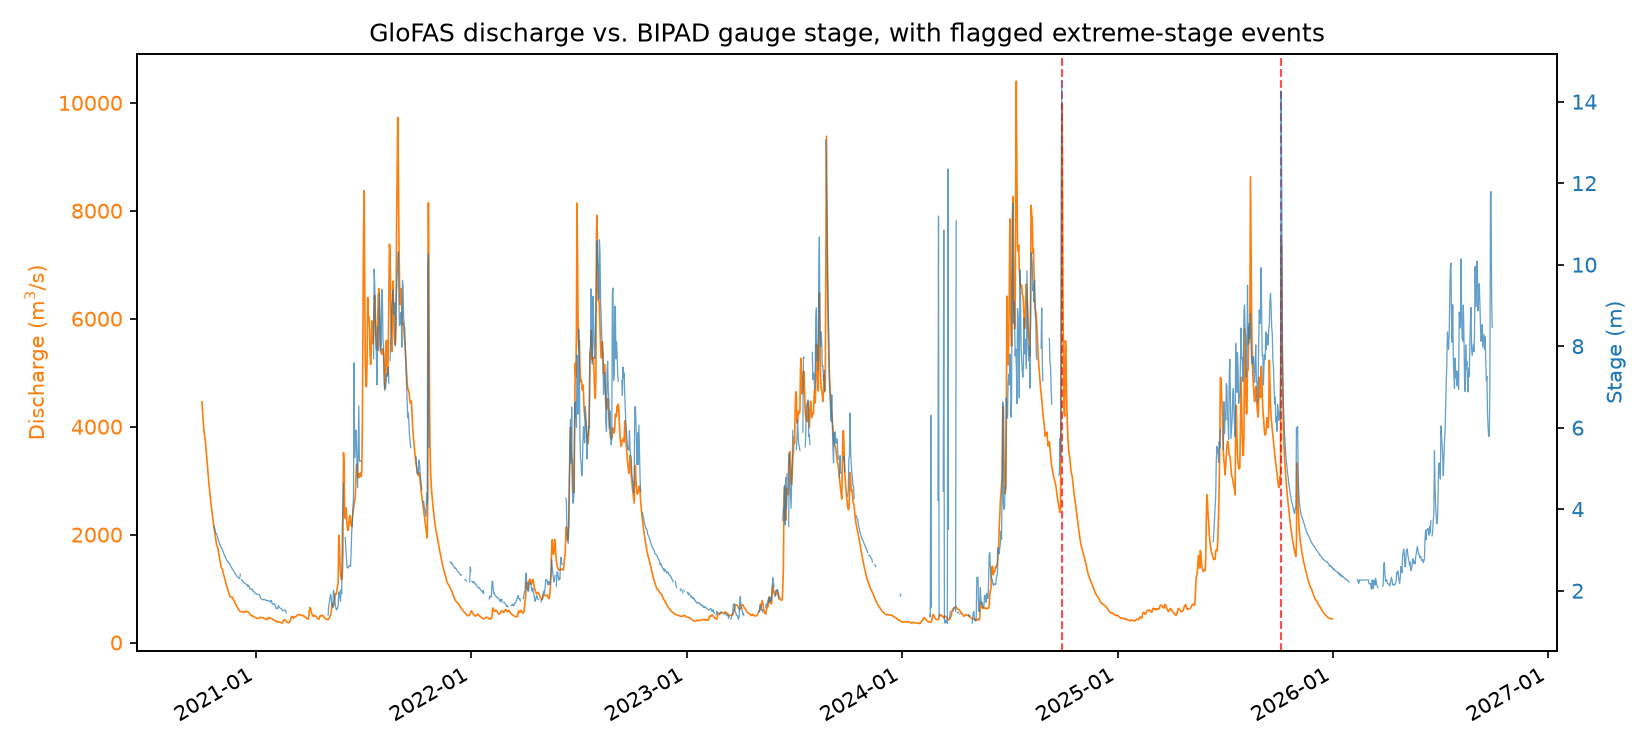
\includegraphics[width=\linewidth]{../analysis/outputs/bipad_glofas_comparison_plot.png}
\caption{GloFAS discharge (Chatara point) vs.\ BIPAD-recorded Hampachuwar stage, 2020--2026, with the two flagged extreme-stage event dates marked.}
\label{fig:bipad}
\end{figure}

\subsection{Rainfall--Discharge Consistency}

As an independent check on the two open datasets underlying this study, basin-mean monthly GPM IMERG rainfall (2001--2025) was compared against monthly-mean GloFAS discharge (1979--2025) over their 297 months of overlap, bounded by the rainfall record's start (Figure~\ref{fig:rainfall-discharge}). The two series track each other closely: Pearson r=0.84 at zero lag, rising to r=0.85 (Spearman $\rho$=0.91) at a one-month lag, then falling to r=0.58 at a two-month lag (all p$<$10$^{-27}$). Both series show a clear, regularly repeating annual monsoon cycle across the ${\sim}$24.75 years of overlap, roughly 25 monsoon cycles, and we read the correlation primarily as a signature of that shared seasonality rather than as clean evidence of a specific basin-response lag: the drop from the one- to two-month lag is faster than a stable routing/storage delay would typically produce for a basin this size, and a shared annual cycle in two independently-derived series will inflate apparent correlation (and understate the true p-value) regardless of any real causal delay between them. This is not a validation of either dataset against ground truth, but it is evidence that the two independently-sourced open datasets used in this study are physically consistent with each other, which is a real (if modest) check that the pipeline is assembling sensible inputs rather than an artifact of the extraction methodology.

\begin{figure}[h]
\centering
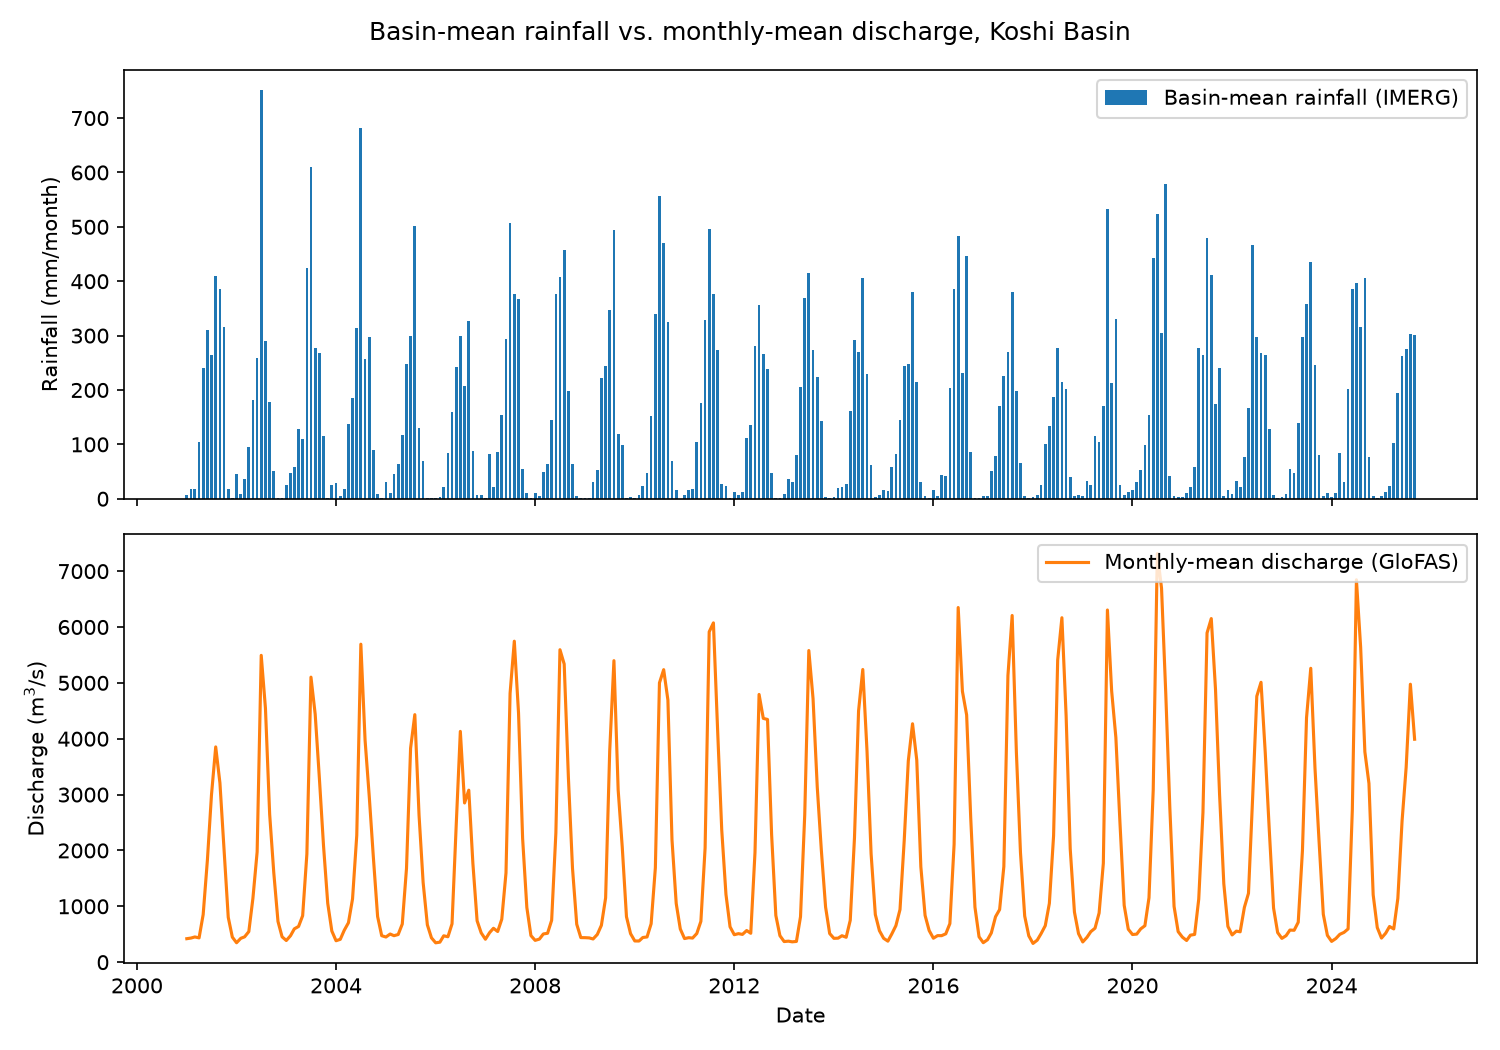
\includegraphics[width=\linewidth]{../analysis/outputs/rainfall_discharge_comparison_plot.png}
\caption{Basin-mean monthly rainfall (IMERG) vs.\ monthly-mean discharge (GloFAS) over their 297 months of overlap, showing a consistent repeating annual monsoon cycle in both independently-sourced datasets.}
\label{fig:rainfall-discharge}
\end{figure}

\subsection{Flood Inundation Mapping}
Using the Gumbel discharge estimates and the hydraulic-geometry depth relation (Section~4.2), inundation depth grows only modestly with return period (4.98\,m at T=10\,yr to 5.60\,m at T=200\,yr, since depth scales with discharge to the 0.3 power in this simplified relation). This single depth is applied uniformly across the whole study area rather than varying with local contributing drainage area, a real simplification, since the outlet gauge's drainage area (53,686\,km$^2$) is roughly three times the upstream gauge's (18,164\,km$^2$), and true local discharge (and hence depth) should scale with local drainage area along the network rather than take one outlet-derived value everywhere; this most likely over-maps extent and depth in upstream reaches relative to the outlet. The resulting maps (Figure~\ref{fig:hand}) show a pattern that is geographically plausible on its face, inundation confined to narrow channels through the hilly northern part of the study area, expanding into extensive, contiguous flooded area across the flat Terai floodplain to the south, where the Sun Koshi/Saptakoshi system exits the Himalayan foothills, but this narrow-in-the-hills/broad-in-the-plains texture is a near-automatic property of HAND itself and should not be read as independent confirmation that the depth values are correct. At T=100 years, an estimated 337,588 DEM cells (${\sim}$304\,km$^2$, roughly 23\% of the ${\sim}$1,320\,km$^2$ study area) are classified as inundated --- figures that inherit the discharge-series bias documented in Section~5.1 and should be read with the same caution.

\begin{figure}[h]
\centering
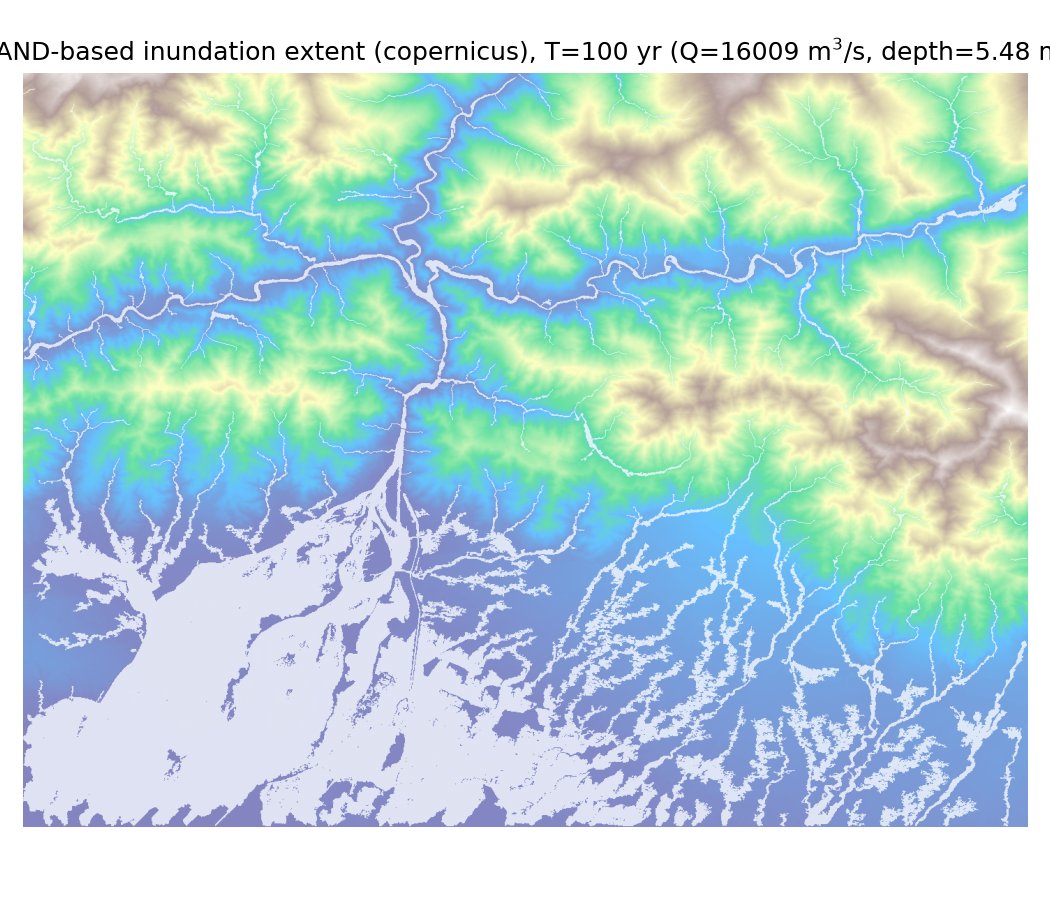
\includegraphics[width=0.85\linewidth]{../analysis/outputs/inundation_map_T100.png}
\caption{HAND-based inundation extent at T=100 yr (Q=16,009\,m$^3$/s, depth=5.48\,m) over the Copernicus GLO-30 DEM. White = classified inundated; note the confined channel flooding in the hilly north vs.\ extensive floodplain inundation in the Terai to the south.}
\label{fig:hand}
\end{figure}

\subsection{DEM Sensitivity: FABDEM vs.\ Copernicus}

To test whether Copernicus GLO-30's known forest/building height bias is materially affecting the flood-mapping result, the identical HAND pipeline was re-run against FABDEM (Forest And Buildings removed DEM, University of Bristol) \citep{hawker2022fabdem}, a machine-learning bias correction of the same underlying Copernicus DEM. FABDEM consistently yields a \textbf{larger} inundated extent at every return period (Table~\ref{tab:fabdem}, Figure~\ref{fig:fabdem}), which is the expected direction: removing canopy/building height lowers the DEM's apparent elevation in vegetated terrain, which lowers HAND values there, pulling more area under the flood-depth threshold.

\begin{table}[h]
\centering
\begin{tabular}{@{}lrrr@{}}
\toprule
Return period (yr) & Copernicus (km$^2$) & FABDEM (km$^2$) & Change \\
\midrule
10  & 291.8 & 300.9 & +3.1\% \\
100 & 303.8 & 312.0 & +2.7\% \\
200 & 306.8 & 314.8 & +2.6\% \\
\bottomrule
\end{tabular}
\caption{HAND-based inundated area, raw Copernicus DEM vs.\ FABDEM.}
\label{tab:fabdem}
\end{table}

\begin{figure}[h]
\centering
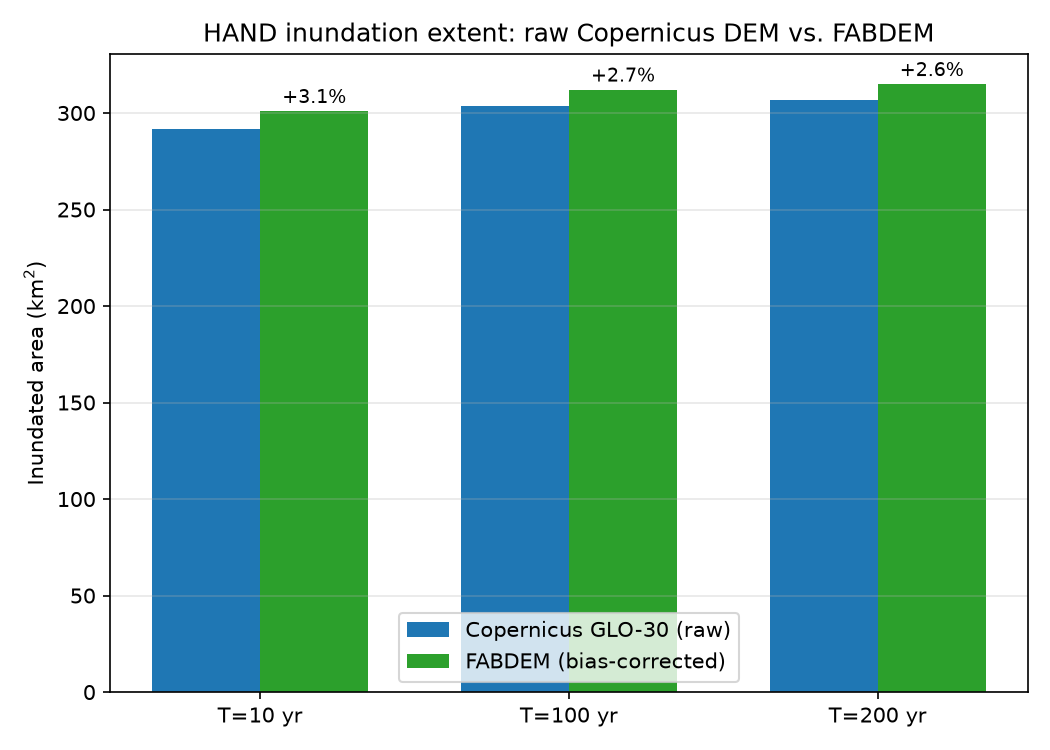
\includegraphics[width=0.85\linewidth]{../analysis/outputs/fabdem_comparison_plot.png}
\caption{HAND inundated area by return period, raw Copernicus DEM vs.\ FABDEM. FABDEM's canopy/building bias correction consistently increases the mapped flood extent.}
\label{fig:fabdem}
\end{figure}

The effect is modest (2.6--3.1\%) but consistent and directionally correct, and it is a genuine, if small, source of uncertainty in the mapping stage that is independent of the discharge/depth-relation uncertainty discussed elsewhere --- a DEM choice, not a hydrology choice, that measurably changes the result. On this evidence FABDEM is the better-justified input for the mapping stage, and we report the Copernicus-based figures elsewhere in Section~5 as the baseline against which this sensitivity is measured. This DEM-driven effect is a real but comparatively minor source of uncertainty next to the ${\sim}$76\% discharge-series bias documented in Section~5.1 --- a reminder that, for this pipeline, the discharge input dominates overall uncertainty far more than the terrain choice does.

\section{Discussion}

\subsection{What this shows}

FLOW's core contribution is demonstrating that this kind of analysis pipeline, flood-frequency analysis feeding GIS-based inundation mapping, can be built and run end-to-end entirely on free global data and open-source software (Copernicus DEM, GPM IMERG, GloFAS, HAND via \texttt{pysheds}), without licensed GIS software or a data-rich basin. The general Gumbel/GIS-mapping method it uses is independently corroborated as viable by a comparable Nepal study on the West Rapti Basin \citep{sharma2025westrapti}, though that study relies on real gauge and terrain data throughout, so it corroborates the method, not FLOW's specific GloFAS-based discharge-sourcing step, which Section~5.1 shows to be unreliable at the individual-event level. The specific numeric results in Section~5 should be read in that spirit: as illustrating what the workflow produces and how its outputs can be checked, not as validated design-flood or inundation-extent values for the Koshi Basin. That distinction is not merely theoretical --- Section~5.1 reports a direct check of the underlying discharge series against a published Chatara gauge record that found it running substantially high (about 76\%) in the one year we could check directly. We consider this a genuinely useful, disclosed finding for other GloFAS-based small-basin studies, not just a caveat about this one, and it is the main reason we describe FLOW's contribution as the workflow rather than the specific numbers it currently produces.

The remaining limitations of the current implementation, the hydraulic-geometry depth relation's generic coefficients and basin-wide application (Sections~4.2, 5.3), the demonstrated GloFAS discharge bias just discussed (Section~5.1), the daily-resolution/flash-flood timescale mismatch (Section~5.1), the self-estimated-parameter limitation on the goodness-of-fit tests (Section~5.1), and GEV's demonstrated unsuitability for this discharge series (Section~5.1), are stated in place where each result is reported, rather than repeated here. Two further points are worth adding at this level: the rainfall input is monthly, adequate for climatological comparison but not for short-lead-time forecasting, a genuine gap relative to where the broader field has moved with ML-based, sub-daily forecasting approaches (Section~2); we consider adding a discharge-forecasting component built on such methods worthwhile future work once an observed discharge record is available, since a model trained against reanalysis discharge rather than observations would be a weaker, partly circular result. And the August 2026 Trishuli disaster, discussed in Section~1 as general motivation, occurred on a different river system and is not itself a validation case for this basin. Section~5.1 reports two events that are: independently-corroborated extreme-stage days on this exact basin (September 2024, October 2025) that GloFAS's discharge series also flags as its year's 2nd-highest day. This checks event \emph{timing}, not magnitude, and the accompanying return-period mismatch, both events are unremarkable (${\approx}$1.6--4.5 years) against the full 47-year climatology despite the danger-level exceedance recorded at both gauges, is itself informative: it shows GloFAS's error here is not a single correctable offset (Section~5.1 already found the opposite-direction problem in 2008, a specific year 76\% too high), a harder failure mode than a consistent bias. This sharpens rather than undermines FLOW's contribution: the pipeline's value is the open, reproducible workflow and the now-characterized ways one of its inputs fails on this basin, not the specific discharge numbers it currently outputs. A genuine quantitative validation still requires a stage-discharge rating curve or real observed discharge for one of these events.

\subsection{Transferability}

Every component of this workflow, a global 30\,m DEM, a global satellite rainfall product, a global discharge reanalysis, and an open-source HAND implementation, is available for any mountain basin on Earth, not only the Koshi. Where a real discharge record (gauge or reanalysis) exists, this workflow can be reproduced end-to-end without licensed GIS software, making it directly applicable to other data-scarce basins across the Himalaya, Andes, or other under-instrumented mountain ranges facing the same monitoring gap. The specific numeric results in Section~5 (Table~\ref{tab:ffa}'s discharge values, Table~\ref{tab:fabdem}'s areas) are local to the Koshi Basin, but the workflow that produced them, data sources, scripts, and method choices, is not.

\section{Conclusion and Future Work}

FLOW demonstrates that low-cost statistical and GIS-based flood analysis, built entirely on free data and open-source tools, is achievable outside the resourcing of a national-scale system like CAFFG, for a real Himalayan basin, and that a direct check of its GloFAS-derived discharge input against published records is itself a necessary and reusable step for any GloFAS-based study of this kind, not an optional one, given the substantial event-level bias we found (Section~5.1). Priority directions for future work: obtaining and incorporating the real DHM discharge record for stations 681/695, now the clearer priority given that demonstrated bias, and more valuable than any other single improvement available to this study; ingesting sub-daily satellite rainfall for genuine short-lead-time forecasting rather than climatological comparison; extending the flood-mapping stage with a surveyed or higher-fidelity channel geometry in place of the empirical hydraulic-geometry approximation; adding an ML-based discharge-forecasting component once real observed data supports it; and obtaining a stage-discharge rating curve for stations 681/695, which would convert the extreme-stage events already identified in Section~5.1 into a quantitative magnitude validation rather than the event-timing check reported here. Further useful extensions, in keeping with FFEWS's original design intent, include critical discharge/precipitation threshold alerts, damage prediction from flood maps combined with demographic data, community alarm routing, and hydrological/bridge design analysis --- several of which are now more tractable given the ML-forecasting literature surveyed in Section~2.

\section*{Data and Code Availability}

All analysis code for FLOW --- the download, flood-frequency, HAND mapping,
rainfall--discharge comparison, DEM-sensitivity, and gauge-stage checking
scripts --- is openly available at
\url{https://github.com/dulalsaurab/Flash-Flood-Early-Warning-Systme-FFEWS}
under the MIT licence, together with the derived result files (return-period
tables, goodness-of-fit statistics, correlation results, and the figures
reproduced in this paper) needed to verify every number reported here without
re-running the downloads. Raw source data is not redistributed: all of it is
publicly available from the providers named in Section~4.2 and is retrieved
automatically by the scripts. Three free registrations (OpenTopography, NASA
Earthdata, and the Copernicus Emergency Warning Data Store) are required to
re-run the download stages; the BIPAD gauge-stage retrieval requires none.
Dataset licences differ from the code licence and are documented in the
repository --- notably FABDEM, which is CC BY-NC-SA 4.0 and therefore
non-commercial only.

\section*{Acknowledgments}

This paper's workflow, FLOW, re-implements the prediction module of FFEWS, a 2014 undergraduate project at the Department of Electronics and Computer Engineering, Institute of Engineering, Tribhuvan University, Nepal, supervised by Dr.\ Sanjeeb Prasad Panday and co-supervised by Deo Raj Gurung (ICIMOD). We also thank ICIMOD and Nepal's Department of Hydrology and Meteorology (DHM) for data access. This study used NASA's GPM IMERG rainfall product, the Copernicus GLO-30 DEM distributed via OpenTopography, the Copernicus Emergency Management Service's GloFAS discharge reanalysis, the University of Bristol's FABDEM \citep{hawker2022fabdem}, and the open-source \texttt{pysheds} library; we gratefully acknowledge these data and software providers.
\bibliographystyle{plainnat}
\bibliography{references}

\end{document}
